%%%%%%%%%%%%%%%%%%%%%%%%%%%%%%%%%%%%%%%%%%%%%%%%%%%%%%%%%%%%%%%%%%%%%%%%%%%%%%%%
%2345678901234567890123456789012345678901234567890123456789012345678901234567890
%        1         2         3         4         5         6         7         8

\documentclass[letterpaper, 10 pt, conference]{ieeeconf}  % Comment this line out if you need a4paper

%\documentclass[a4paper, 10pt, conference]{ieeeconf}      % Use this line for a4 paper

\IEEEoverridecommandlockouts                              % This command is only needed if 
                                                          % you want to use the \thanks command

\overrideIEEEmargins                                      % Needed to meet printer requirements.

% See the \addtolength command later in the file to balance the column lengths
% on the last page of the document

% The following packages can be found on http:\\www.ctan.org
%\usepackage{graphics} % for pdf, bitmapped graphics files
%\usepackage{epsfig} % for postscript graphics files
%\usepackage{mathptmx} % assumes new font selection scheme installed
%\usepackage{times} % assumes new font selection scheme installed
%\usepackage{amsmath} % assumes amsmath package installed
%\usepackage{amssymb}  % assumes amsmath package installed
\usepackage{wrapfig}
\usepackage{graphicx,color}

\usepackage{textcomp}
\usepackage{amsmath}
\usepackage{cases}
\usepackage{xspace}
%\usepackage{algorithm}
%\usepackage{algorithmic}
\usepackage{graphicx}
\usepackage{caption}
\usepackage{subcaption}

%EDITING COMMANDS
\newcommand{\hilight}[1]{\colorbox{red}{#1}}
\newcommand{\todo}{\colorbox{red}{TODO}}

\title{\LARGE \bf
WORKING TITLE: Incorporating User Feedback in Motion Planning for Manipulators
}


\author{Arjun Menon$^{1}$, Sachin Chitta$^{1}$, Mark Moll$^{2}$, Lydia Kavraki$^{2}$% <-this % stops a space
\thanks{*This work was supported by ...}% <-this % stops a space
\thanks{$^{1}$SRI International, Menlo Park, CA
        {\tt\small arjun.menon@sri.com, sachin.chitta@sri.com}}%
\thanks{$^{2}$Rice University, Department of Computer Science, Houston, TX
        {\tt\small mmoll@rice.edu, kavraki@rice.edu}}%
}


\begin{document}



\maketitle
\thispagestyle{empty}
\pagestyle{empty}


%%%%%%%%%%%%%%%%%%%%%%%%%%%%%%%%%%%%%%%%%%%%%%%%%%%%%%%%%%%%%%%%%%%%%%%%%%%%%%%%
\begin{abstract}

Co-robots, i.e. robots that need to work close to people, will need to account for the preferences and expectations of their human 
co-workers in executing motions or actions. Consistent, legible and predictable motions are a key factor in making humans comfortable 
around robots. In this work, we take a first step towards designing motions that are more acceptable to human co-workers by asking 
people to rate robot motions generated in a variety of environments. Our approach is data-driven, i.e. we aim to use data from an online 
survey to inform good quality paths and trajectories. We compute a set of features for each trajectory and use the features 
and associated ratings to try add predict a quality score that represents how well the human observers liked the trajectory. We present an 
analysis of the dataset that we have collected, highlighting the features that dominate the trajectories that people prefer. We also 
present a classifier that will return the quality score for a given trajectory. Finally, we discuss how a data-driven approach using the 
results of this analysis can be used to help design better plans that are more acceptable to people. 
\end{abstract}


%%%%%%%%%%%%%%%%%%%%%%%%%%%%%%%%%%%%%%%%%%%%%%%%%%%%%%%%%%%%%%%%%%%%%%%%%%%%%%%%
\section{INTRODUCTION}

Robots working in industrial environments have traditionally been limited to simple, efficient point to point motions. Robotic workcells 
typically require a safety cage to prevent people from being getting close. Robotic motion generation, therefore, does not take 
into account any notion of the acceptability of motions for human observers. The need for more flexibility in manufacturing and logistics, 
though, has resulted in a greater need for robots that can work beside humans. As robots and people start becoming co-workers, taking 
human perception of robotic paths into account will become more important. Humans are able to predict and adjust their motions to 
account for the expectations and motions of their co-workers easily. For human co-workers to be comfortable, robots will similarly 
have to tailor their motions for the presence and actions of the people around them. 

In this work, we take a first step towards the ultimate goal of generating robotic arm motions in cluttered environments that are acceptable for human observers and co-workers. We start with a survey where human observers rate robot motion quality. We generated a range of trajectories across multiple environments with different planners. The motion planning problems we chose required a (simulated) robot to move its arm from a specified end-effector start position to a desired end-effector goal position. Movies of these trajectories from multiple viewpoints were then presented to human observers using an online survey tool. The users were asked to rate different attributes of the trajectories. We also computed a large set of features for each trajectory. The feature set was designed to be easily extensible across different types of robots and also captures the relationship between the trajectories and the environment. We use the feature set, coupled with machine learning techniques, to build a classifier that predicts the human rating for a given trajectory. The classifiers also help in identifying a set of features that are the most important in predicting human preferences for robot trajectories. The classifiers could also form the basis for a new {\em data-driven} approach to motion planning. 

This paper is organized as follows. In Section~\ref{sec:background}, we first describe some of the existing approaches to designing better quality paths for robots. We also look at how human motion information has inspired work in designing better trajectories for robots. In Section~\ref{sec:survey}, we present details of the online survey including information about the types of trajectories and environments used. Section~\ref{sec:raw_results} presents raw results from the survey, including examples of trajectories that were rated well and badly. In Section~\ref{sec:analysis}, we present a set of features corresponding to the trajectories and use a machine learning approach to derive a classifier for predicting the rating of trajectories. In Section~\ref{sec:conclusion}, we conclude with a discussion of how our results could be used to design motion planners that generate more human-acceptable trajectories. 

\begin{figure*}
\centering
\begin{subfigure}[b]{0.3\textwidth}
    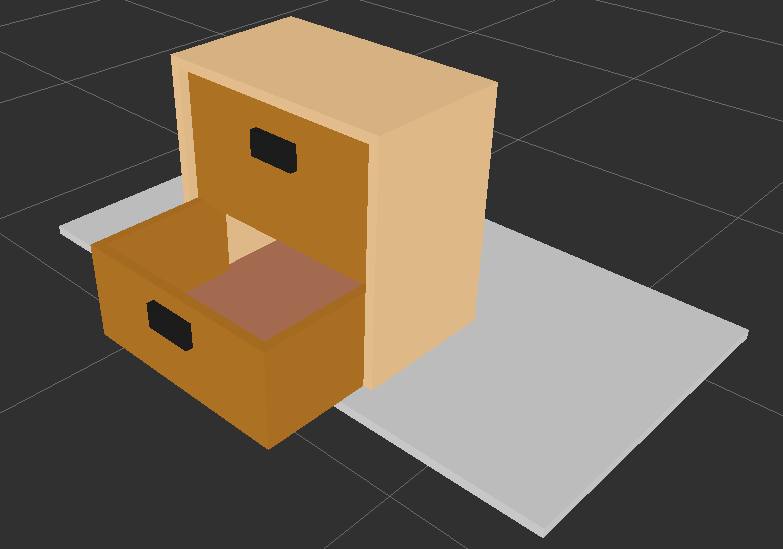
\includegraphics[trim = 0mm 0mm 0mm 0mm, width=\textwidth]{pictures/drawer_scene}
    \caption{}
    \label{drawer_scene}
  \end{subfigure}%
  ~ %add desired spacing between images, e. g. ~, \quad, \qquad etc.
%(or a blank line to force the subfigure onto a new line)
  \begin{subfigure}[b]{0.25\textwidth}
    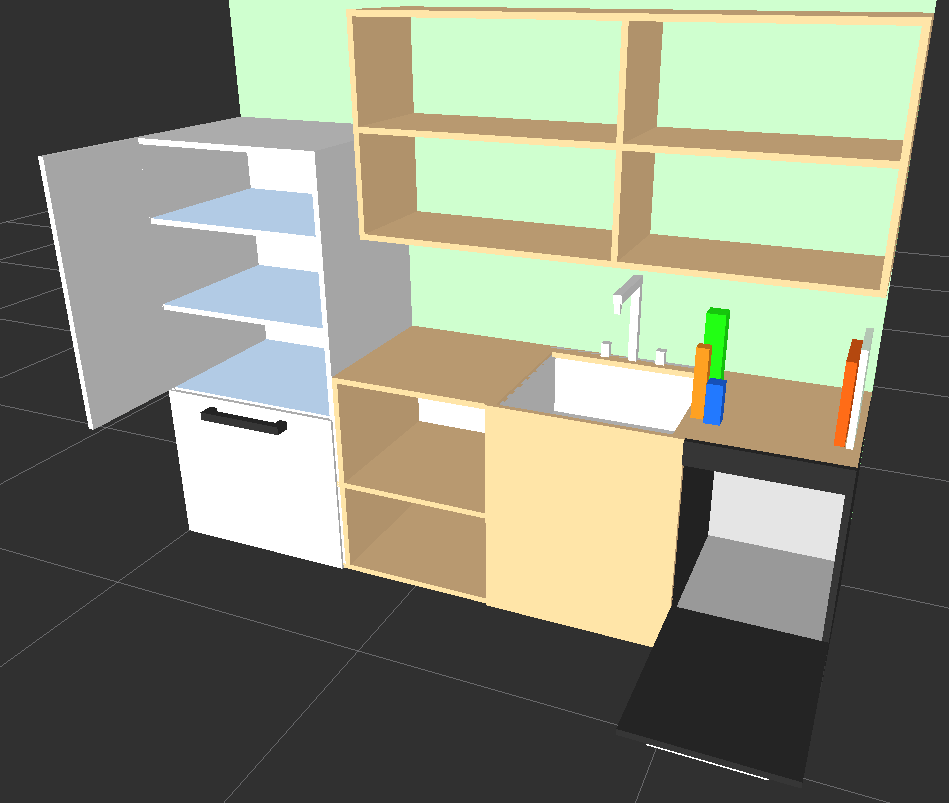
\includegraphics[trim = 0mm 0mm 0mm 0mm, width=\textwidth]{pictures/countertop_scene}
    \caption{}
    \label{fig:countertop_scene}
  \end{subfigure}
  ~ %add desired spacing between images, e. g. ~, \quad, \qquad etc.
%(or a blank line to force the subfigure onto a new line)
  \begin{subfigure}[b]{0.38\textwidth}
    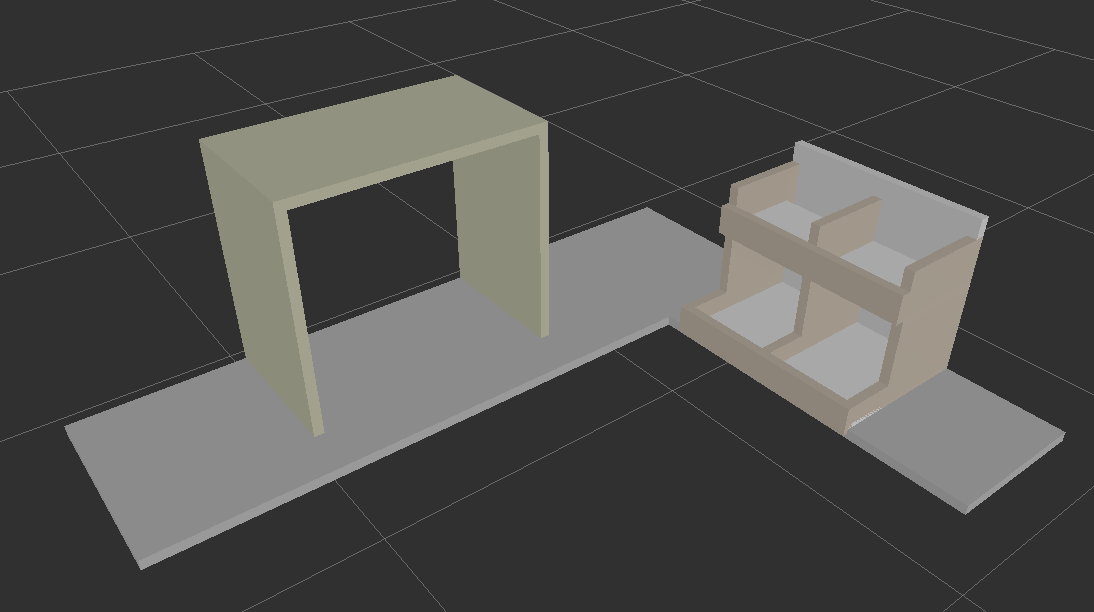
\includegraphics[trim = 0mm 0mm 0mm 0mm, width=\textwidth]{pictures/industrial_scene}
    \caption{}
    \label{fig:industrial_scene}
  \end{subfigure}
\caption{The scenes used in generating the library of robot motions to collect feedeback for. (a) \emph{Drawer} (b) \emph{Countertop} and (c) \emph{Industrial}}\label{fig:scenes}
\end{figure*}

\section{Background}
\label{sec:background}

Robot motion study for industrial has been primarily influenced by the need to generate smooth jerk-free trajectories that minimize wear and tear of internal parts. In recent years, there has been more interest in the generation of motions for robots working in human environments, i.e. environments with clutter and people working next to the robots. Most attention, though, has been focused on generating {\em collision-free} motions. Examples include the use of randomized planners\cite{kuffner_RRT_icra00}, trajectory optimization techniques\cite{Mrinal:2011}, and deterministic search-based techniques\cite{Cohen:2012}. Such approaches have also been modified to account for other types of constraints, e.g. dynamic constraints or process constraints arising from the task. 

Human motions have been the subject of recent stufy with the intent of determining whether there are certain motor or locomotor invariants that best describe human manipulation or locomotion. Human motion has been observed to be stereo-typical~\cite{Atkeson:85}, i.e. learned motion patterns that are repeatedly used. This requires less planning of individual motions and contributes to making human motions more deterministic and predictable. The minimum jerk principle for human motions specifies that the trajectory of the human can best be represented as a motion that minimizes jerk of the hand~\cite{Flash:85}. Uno et. al.~\cite{Uno:89} used minimum torque change as a measure to explain the observed human motions. Minimizing jerk at the joint level~\cite{Rosenbaum:1995} has been another criterion used for human motion. Human motion has also been found to be optimized~\cite{Arechavaleta:2006}. Albrech et. al.~\cite{Albrecht:2011} studied the reaching motions of several subjects in table-setting situations and attempted to codify the motion using cost functions representing minimum-jerk hand motions, minimum-jerk joint motions, minimum torque change and a combination of all three. They found that no single combination of the cost functions explained the observed data completely. 

Recent work has also addressed the task of making motions predictable (similar motions in similar environments and tasks) and/or legible (make it easier for human observers to understand the intent of the robot)~\cite{Beetz:2010}. Legibility makes it possible for human observers to understand clearly what a robot is intending to do, allowing them to modify their actions and motions if necessary. Predictability implies that the robot will always be consistent in its actions, removing the element of surprise for human observers. These concepts have been well-studies recently with the intent of measuring legibility~\cite{Lichtenthaler:2011}, using expressions to improve the readability of robots~\cite{Takayama:2011} and generating anticipation~\cite{Gielniak:2011}. In~\cite{Dragan:2013}, the notion of legibility was incorporated into a constrained trajectory optimization motion planner to generate motions that are more legible to human observers. 

There has been relatively little examination of how human observers perceive robot arm trajectories in environments with obstacles. There is no data available for how human observers react to such robot motions. It is not clear whether minimum-jerk trajectories (or other cost functions) are the best descriptors of motions in such environments or if there are other features that better explain human-observer preferences in such sitations. Our goal in this work is to collect the data needed to answer the query, "Which robot trajectories in cluttered environments do human-observers prefer". A second question that we would like to answer is "Why are certain robot trajectories preferred by human-observers?". This is a larger question that we aim to address in future work and instead we focus on,"Can we predict a human-observer preference for a given trajectory". The answer to this latter question, we hope, will eventually point us towards a cost function for generating more human friendly motion plans. 

\section{Approach}
\label{sec:survey}
Our approach starts with an online survey designed to get information from multiple users about how well they like robot trajectories. In this section, we will describe in detail the infrastructure used to create the trajectories and movies that were used in the survey and the online 
survey procedure used. 

\subsection{System Infrastructure}

In order to quickly produce a large number of robot trajectories, the MoveIt benchmarking architecture~\cite{cohen2012generic} was extended with video recording capabilities. Every trajectory was generated by a combination of \emph{scenes}, \emph{queries}, and \emph{planners}. In this paper, our trajectories are planned in three distinct scenes (shown in~\ref{fig:scenes}) which the robot can interact in: a kitchen (\emph{Countertop}), an industrial workbench (\emph{Industrial}) and a drawer on a table (\emph{Drawer}).

\begin{figure}[b]
    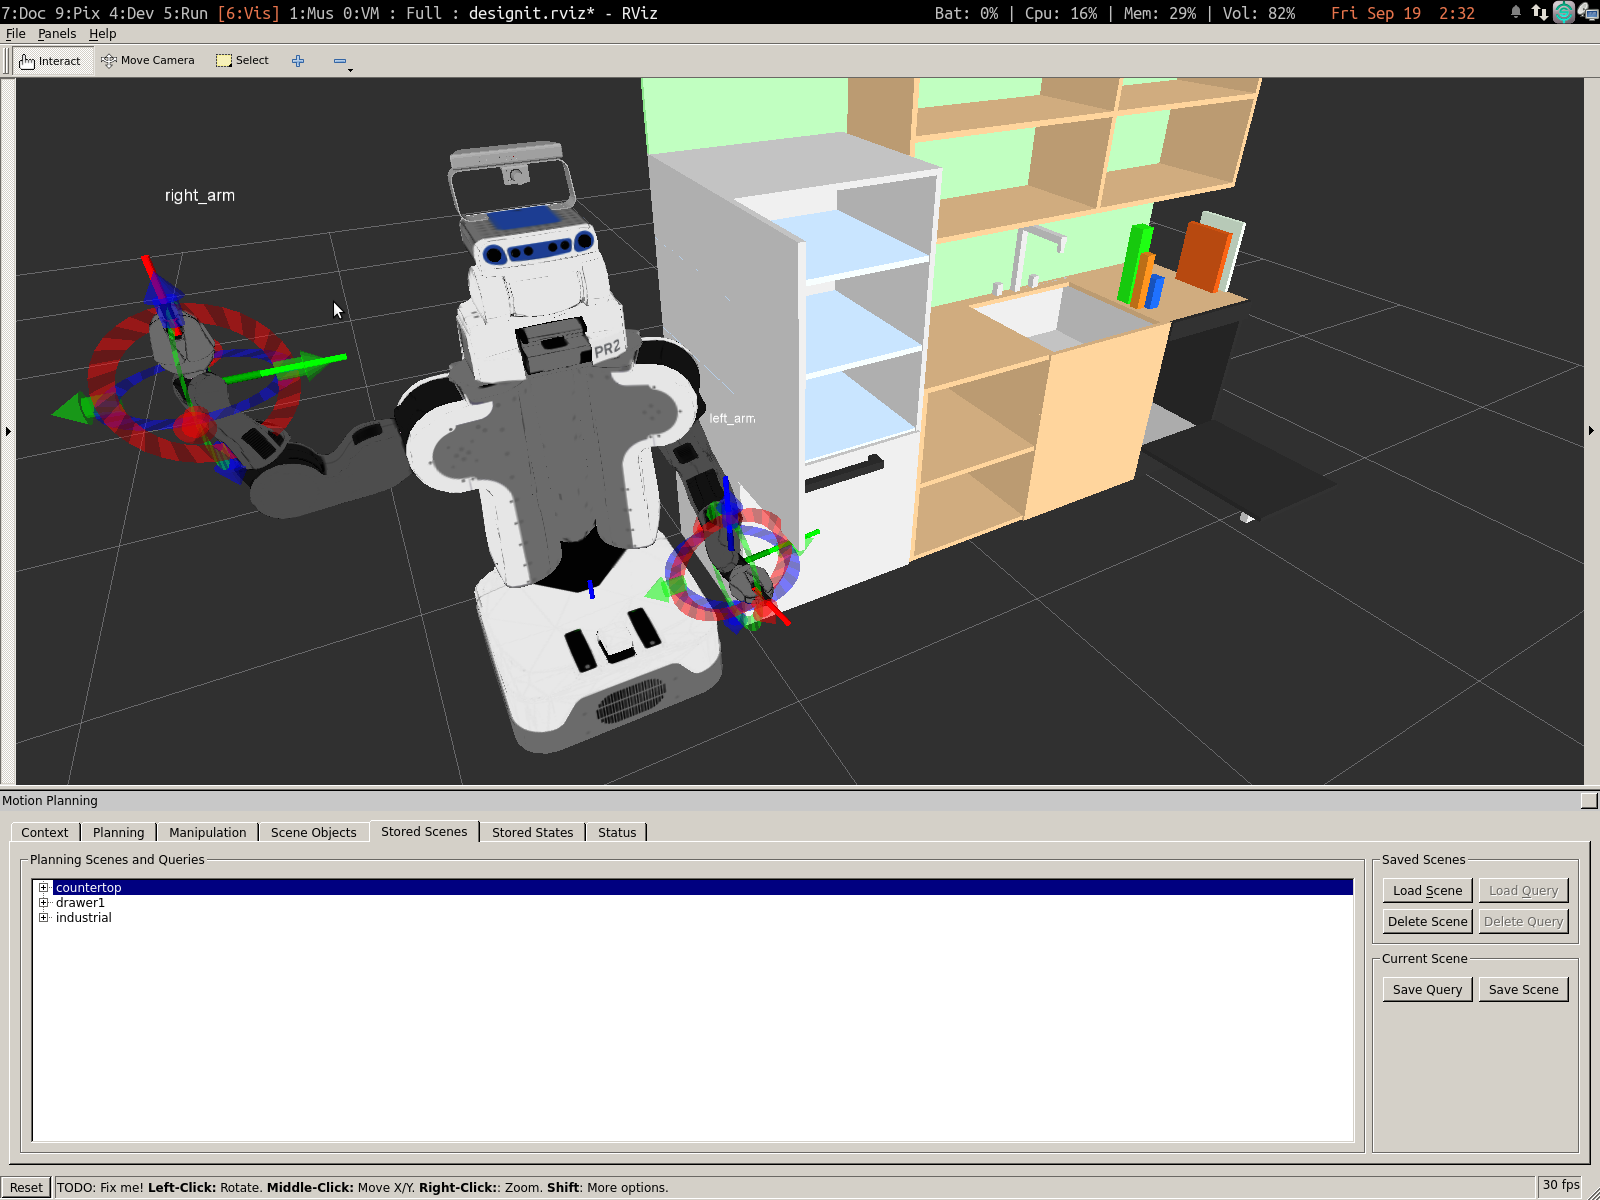
\includegraphics[trim = 0mm 0mm 0mm 0mm, width=\columnwidth]{pictures/designing_queries_moveit}
    \caption{Screenshot of the planning query design process which involved hand-picking start and goal query poses for the various scenes manually to ensure they were neither trivial nor impossible for the planning algorithms to solve. This was accomplished through use of RVIZ and interactive markers.}
    \label{fig:design}
\end{figure}

After selecting the scenes, the robot was positioned in the scenes manually and planning queries were constructed by hand to reach a requisite number of planned trajectories~\ref{fig:design}. The positioning in the scenes was done with the expectation that the planning queries would not be impossible or trivial for the planning algorithms to solve. 

Finally, the planning algorithms that were used were RRT-Connect~\cite{kuffner2000rrt}, and RRT*~\cite{frazzoli-RRTstar} with two cost functions: \emph{PathLength} and \emph{MaxMinClearance}.The objective for \emph{PathLength} minimizes the length of the trajectory (as the sum of the euclidean distances between ends of trajectory segments). The objective for \emph{MaxMinClearance} computes uses the minimum clearance of a configuration belonging to a trajectory as the value it is trying to maximize.

The library of trajectory videos was collected by computing plans with each of the previously discussed planners for the planning queries and scenes hand-picked from above. The plans were then recorded in simulation through RVIZ. In designing the online survey, these video recordings would be taken from multiple vantage points to maximize the visibility of the motion to the participant reviewing it.

\subsection{Online Survey}

\begin{figure}
    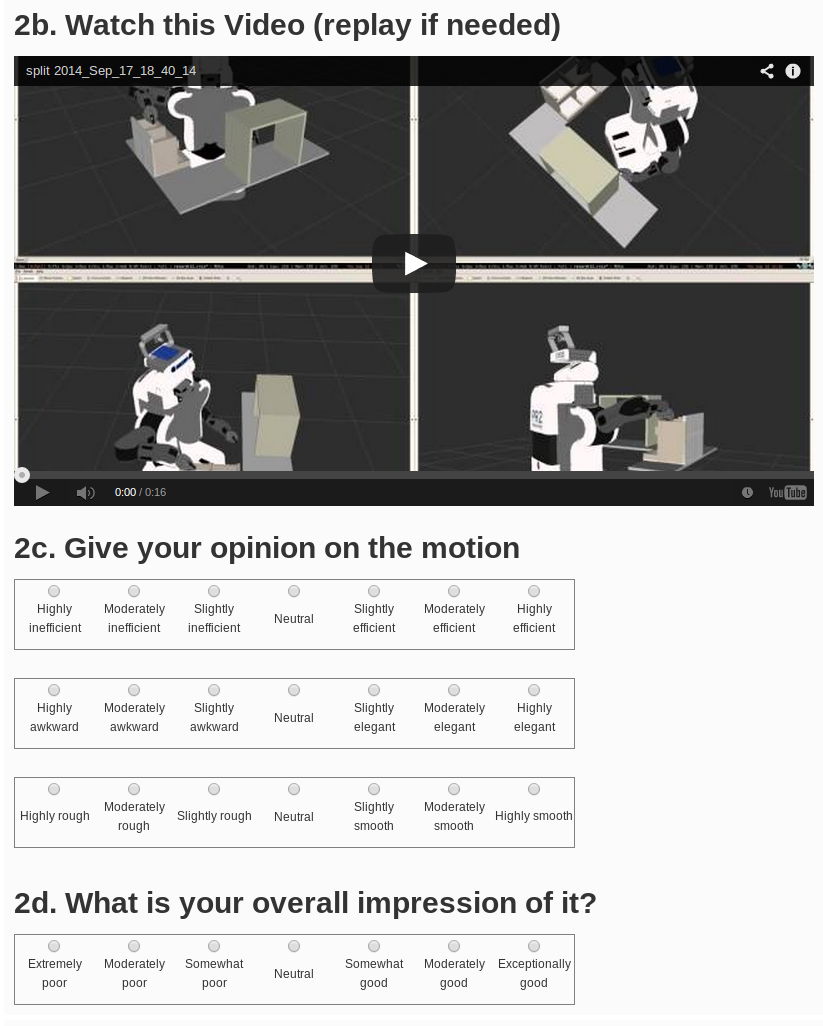
\includegraphics[trim = 0mm 0mm 0mm 0mm, width=\columnwidth]{pictures/amazon_survey_screenshot}
    \caption{The main survey question which prompts the participant for a rating in four motion characteristics (efficiency, elegance, smoothness and overall impression) after presenting a video that demonstrates the motion from four clearly visible vantage points for any sample trajectory.}
    \label{fig:survey_question}
\end{figure}

Each participant was allowed to provide feedback no more than once for each of the trajectories generated by the survey design. We ran the survey for 103 trajectories, requesting no more than 20 ratings per trajectory. Participants are allowed to rate multiple distinct trajectories, but no more than once.The analysis of these results will be done in Section~\ref{sec:analysis}.

\subsubsection{Demographic Questions}

Participants were asked a few demographic questions which ask about:

\begin{itemize}
\item Familiarity with videogames
\item Familiarity with robotics
\item The participant's age group: We asked whether the participant belonged to the 18-24, 25-44, 45-64, and 65+ age brackets.
\item The participant's highest education level: We asked if the particpant had a PhD/Masters, a Bachelors, Associate or High School level degree as their highest education.
\end{itemize}

None of these pieces of information were used to filter the responses we collected.

\todo find info on relation between videogame and robotics

\subsubsection{Survey Design and Process}

The surveys were presented to users of Amazon Mechanical Turk~\cite{paolacci2010running}, who would be presented with a set of demographic questions, a video, and the four scales to rate the robot's motion on the basis of elegance, efficency, smoothness and overall impression. Additionally a control question was presented with another video asking the participant about the robot's action in the accompanying video. This served as the first satisficing trap to ensure that participants were truthfully attempting the survey. On overview of the main survey question can be seen in Figure~\ref{fig:survey_question}.

Mechanical Turk allows dispensing of monetary compensation on completion, which was set to 15\textcent~ per survey. The expected time to complete was 1-2 minutes, which allows the participant about 1 whole minute of deliberation when assigning ratings. Additionally, the participants were allowed to replay the trajectory video repeatedly (and other features that Youtube supports). This maximum possible payout is 15.45\textdollar~ or if each survey took on average 1.5 minutes to complete about 6\textdollar~ per hour of work for a participant.

\begin{figure}
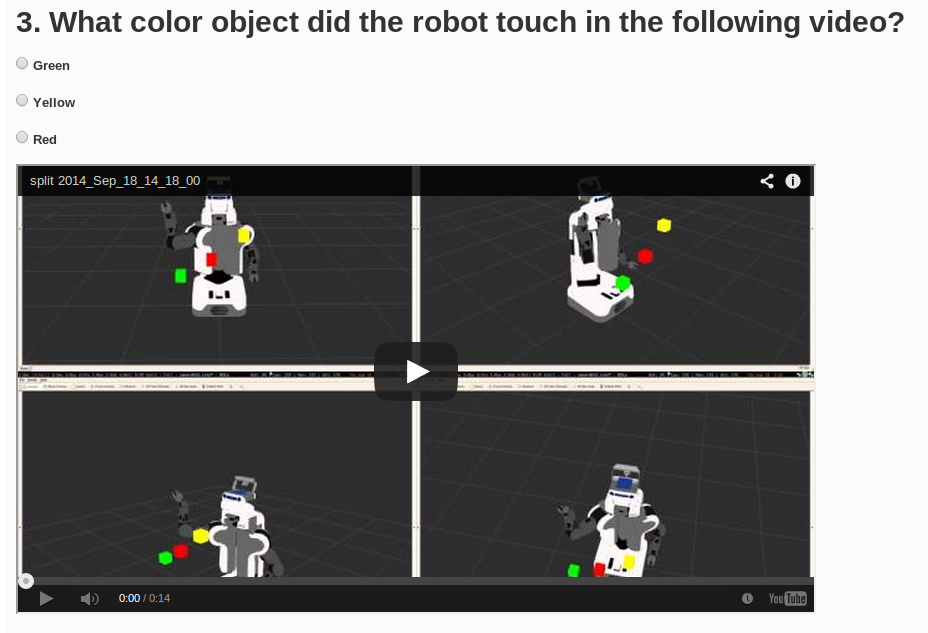
\includegraphics[trim = 0mm 0mm 0mm 0mm, width=\columnwidth]{pictures/amazon_control_question}
\caption{The survey control question which prompts the participant about the action of the robot in the accompanying video. The question we adopted was to ask the particpant which colored cube the robot touched.}
\label{fig:control_question}
\end{figure}

In addition to the rating and demographic questions, a control question was incorporated to account for satisficing in online surveys~\cite{krosnick1991response}~\cite{krosnick1996satisficing}. The question format can be seen in Figure~\ref{fig:control_question}. This question served as the first counter-measure against satisficing in the survey. The other counter-measure was to manually inspect the responses, and assess whether it agrees with the other survey respondents on a participant-by-participant and then trajectory-by-trajectory basis. The process for examining a particular participant involves seeing how his/her ratings agree or disagree with the average ratings of all the other ratings for this particular trajectory. Aggregating this over all the trajectories the participant rated gives us an idea of how much we can trust their responses and make a decision about rejecting all or none of their responses. Another heuristic we employed in inspecting the responses was looking for the average time to complete the survey to be extremely low, which could hint at strong satisficing.

\section{Survey Results}
\label{sec:analysis}
The results of the survey are summarized in Fig.~\ref{fig:survey_raw} which shows a histogram of (average) responses for each of the four survey questions across the 100 trajectories that were rated by users. It is clear that a majority of the trajectories in our survey were well received by the human observers but there were quite a few trajectories that were rated badly as well. 
\begin{figure}[t]
  \centering{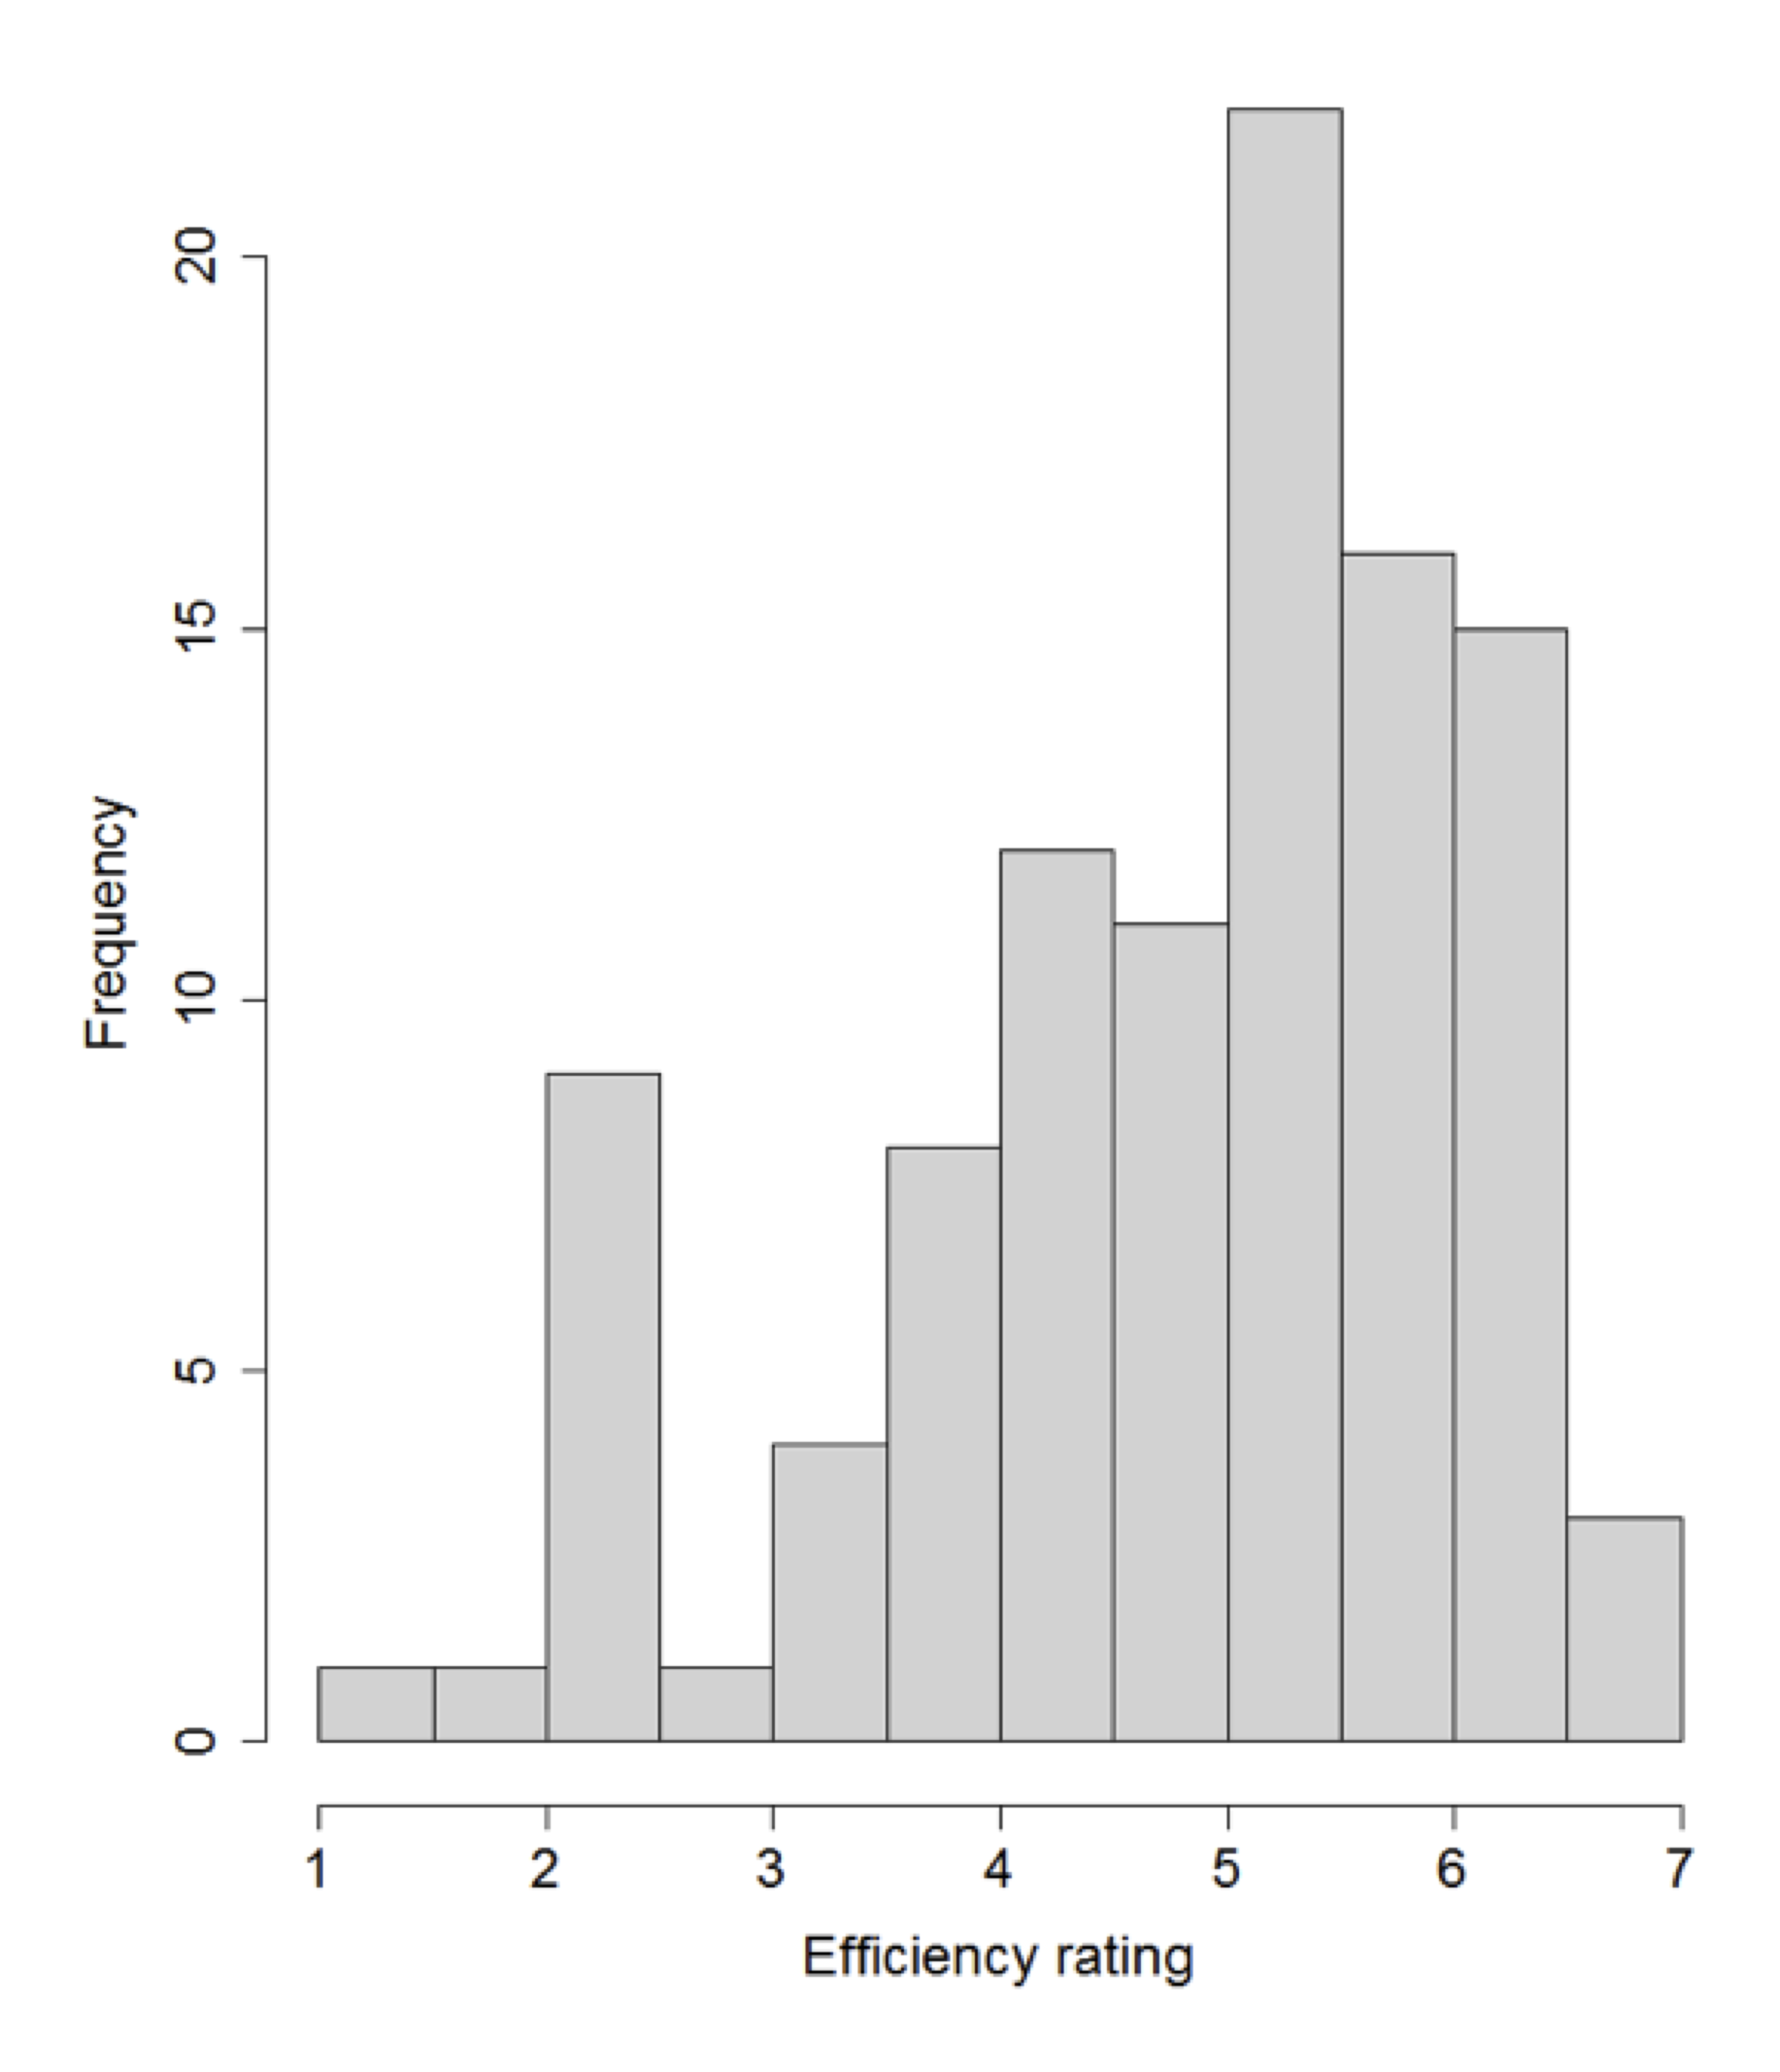
\includegraphics[width=0.45\linewidth]{pictures/efficiency}}
  \centering{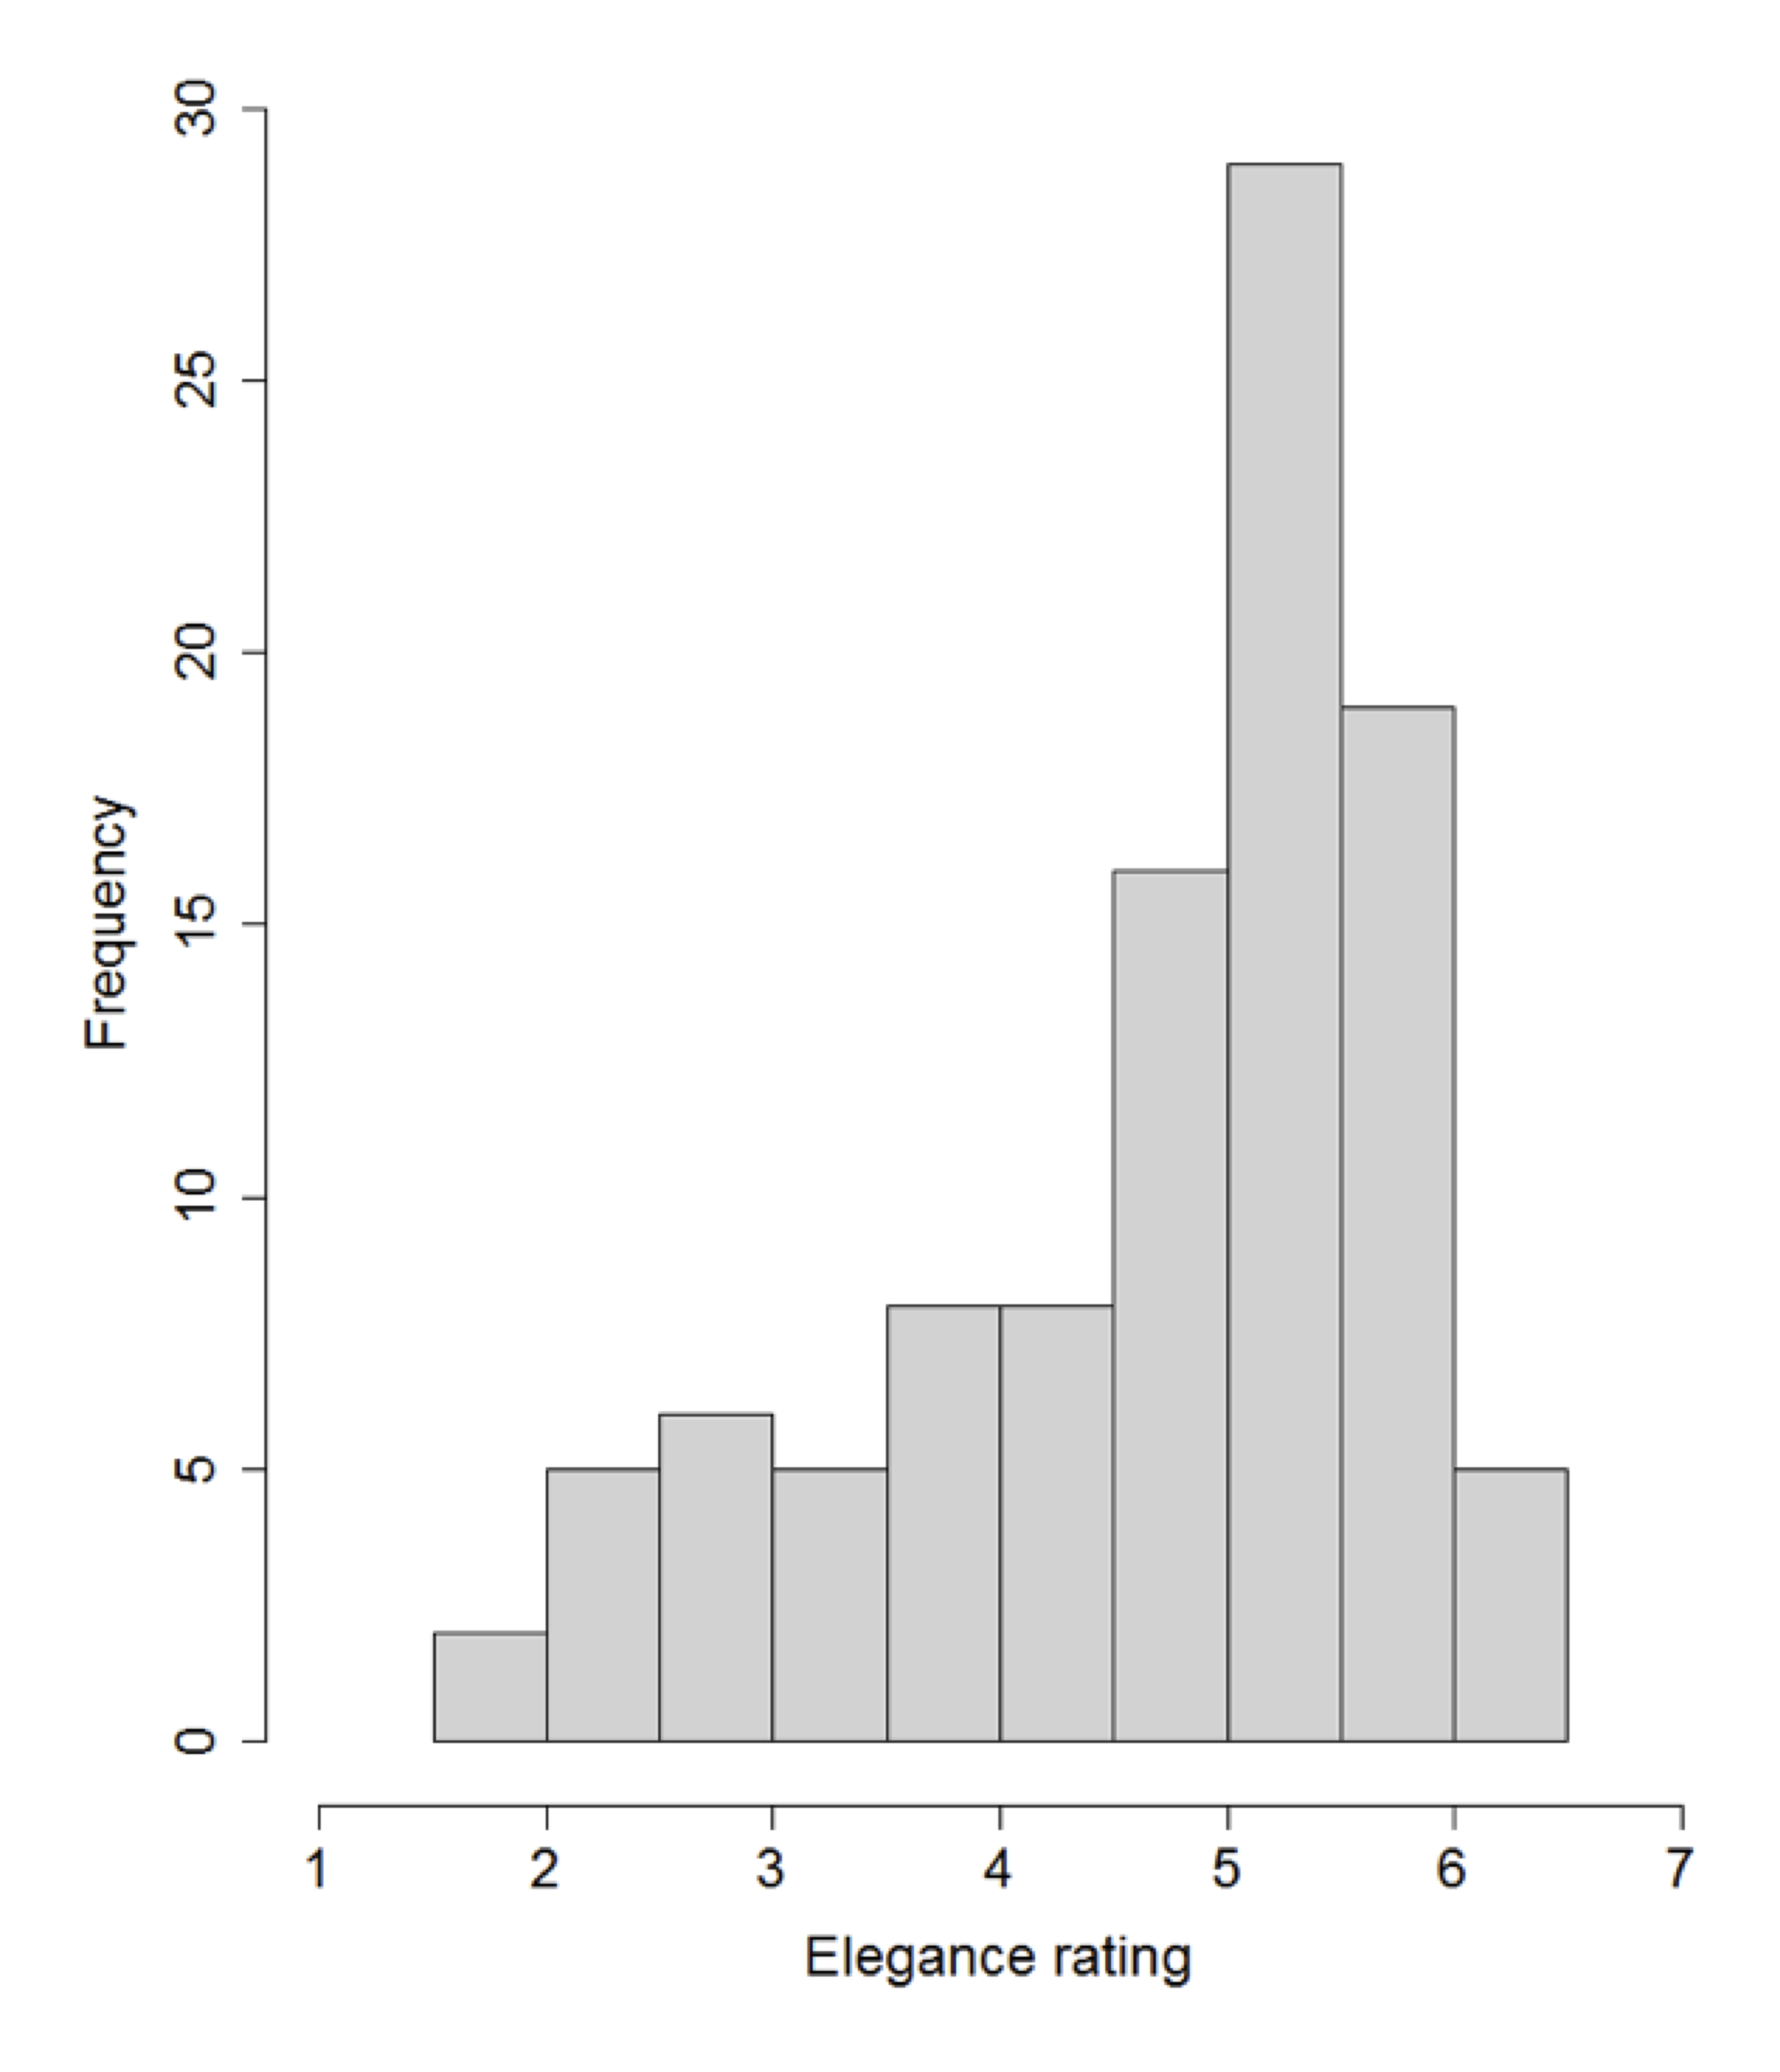
\includegraphics[width=0.45\linewidth]{pictures/elegant}}
  \centering{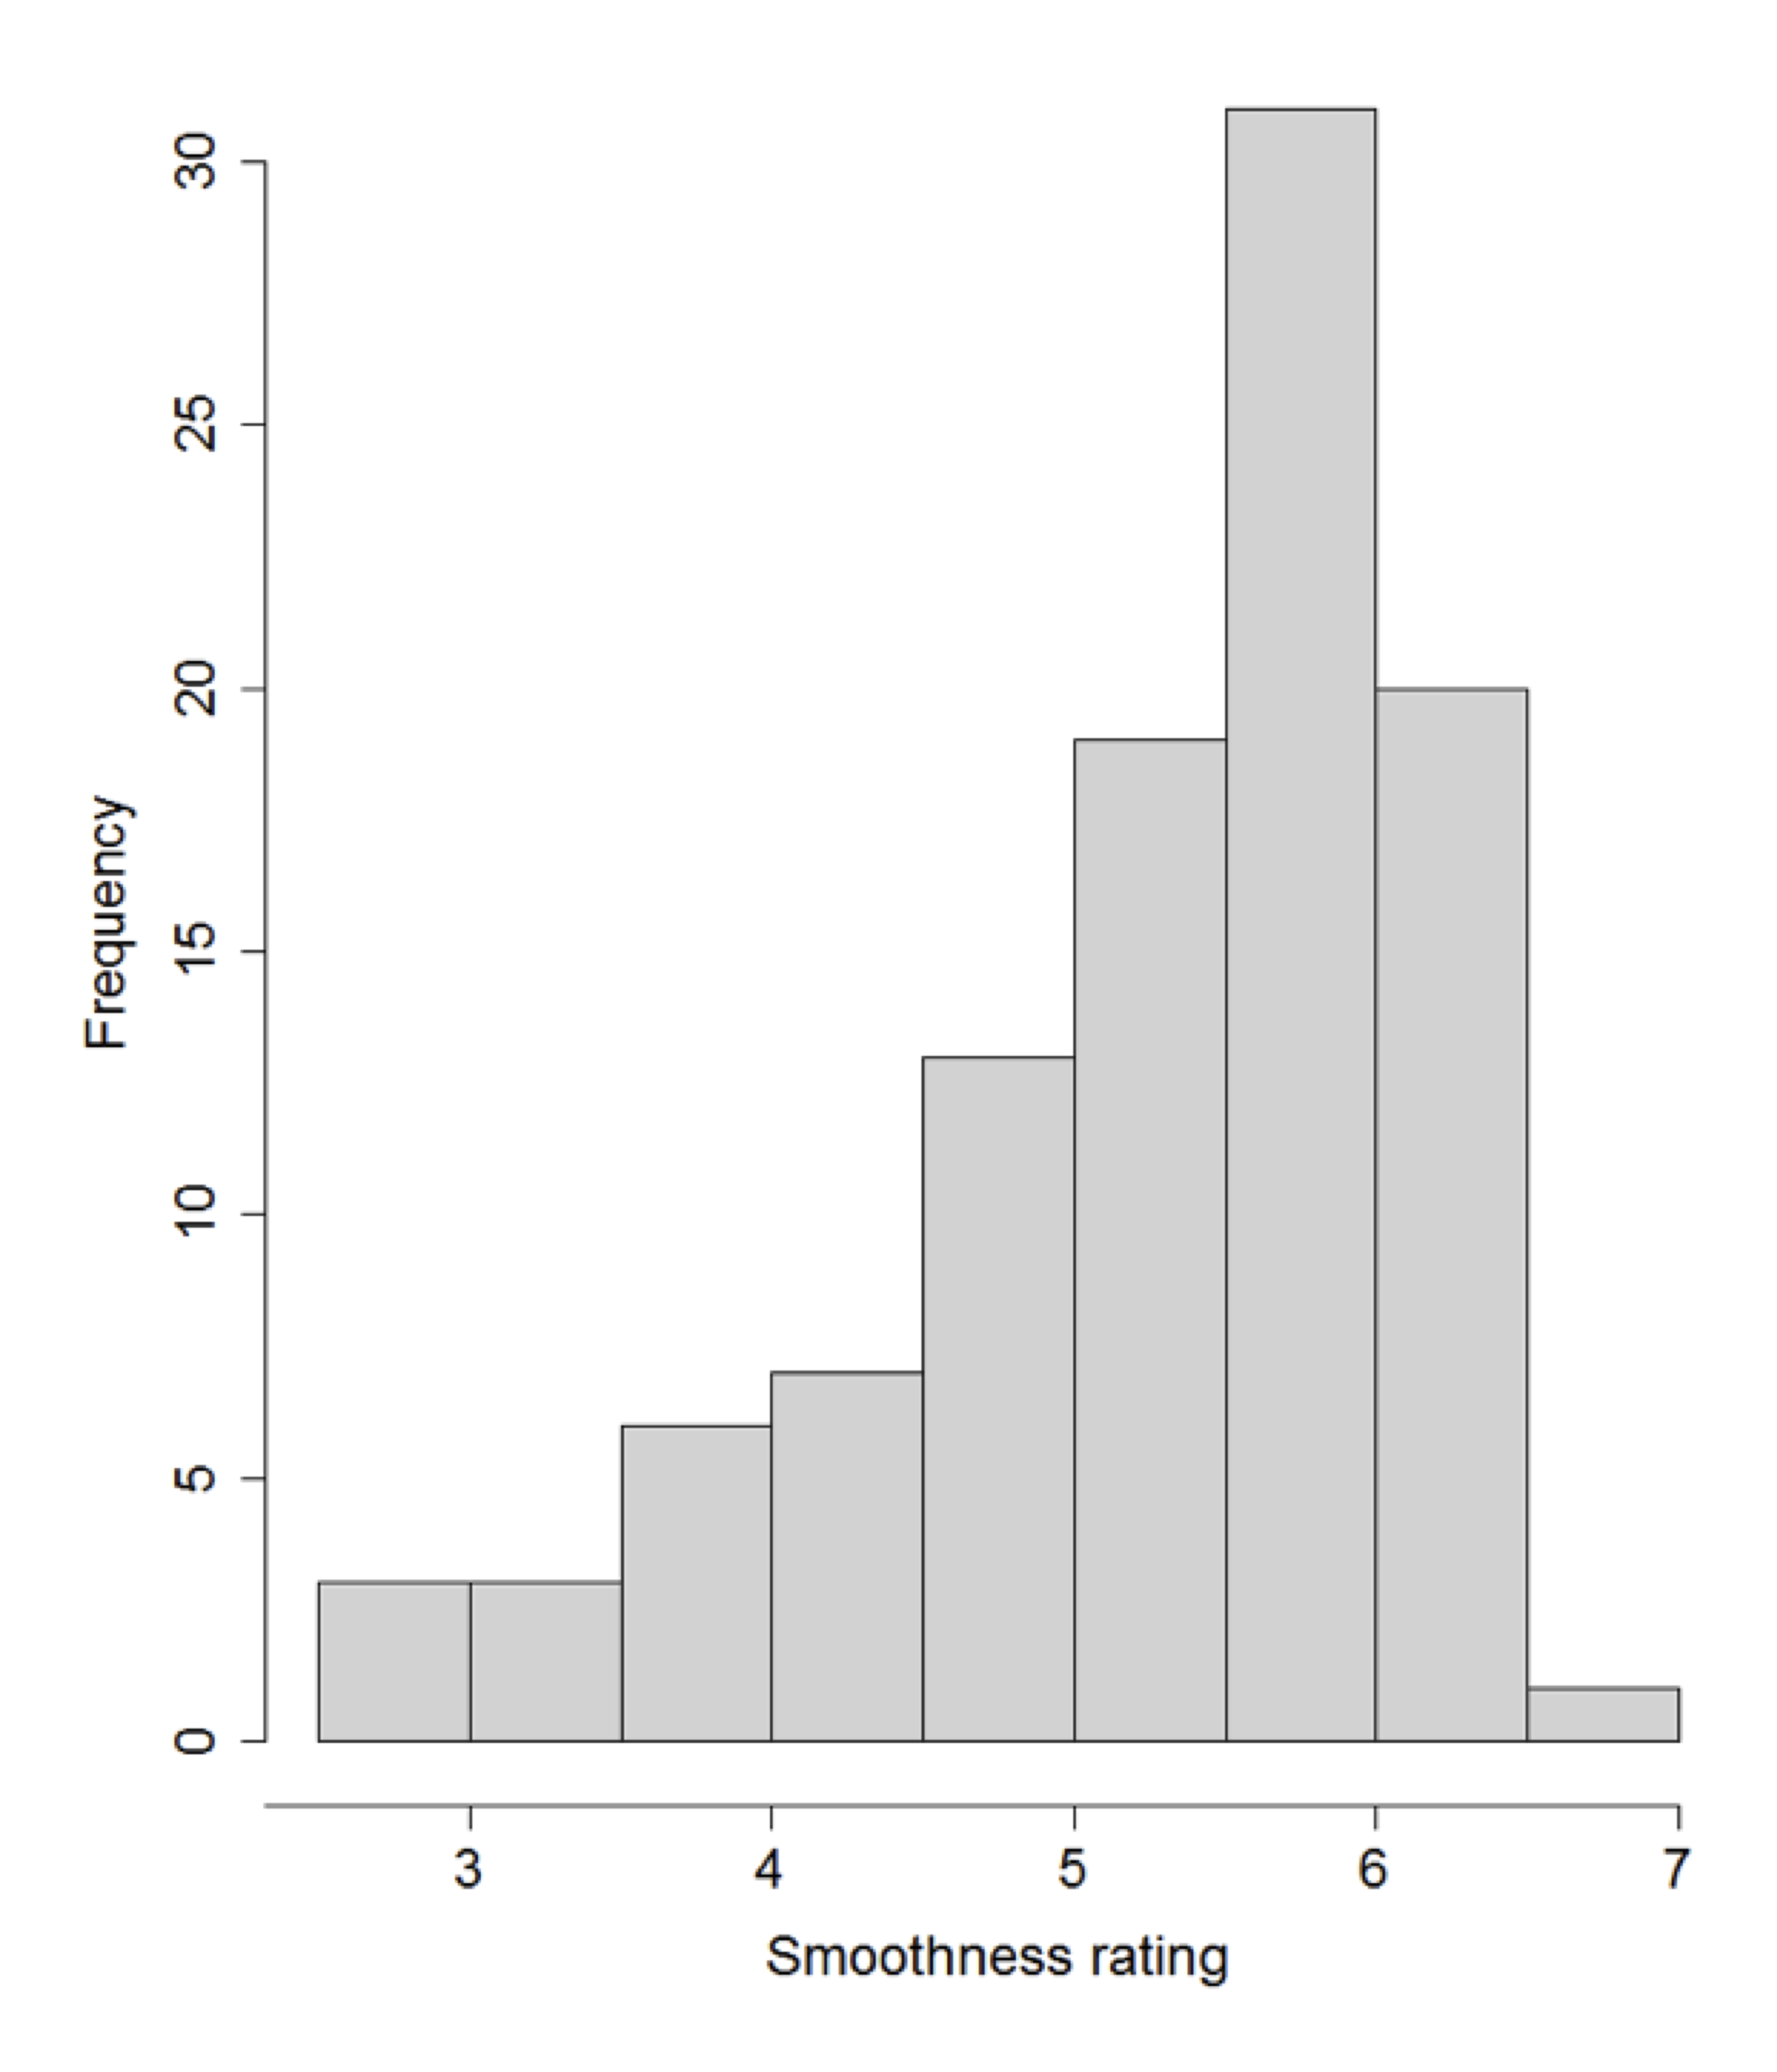
\includegraphics[width=0.45\linewidth]{pictures/smooth}}
  \centering{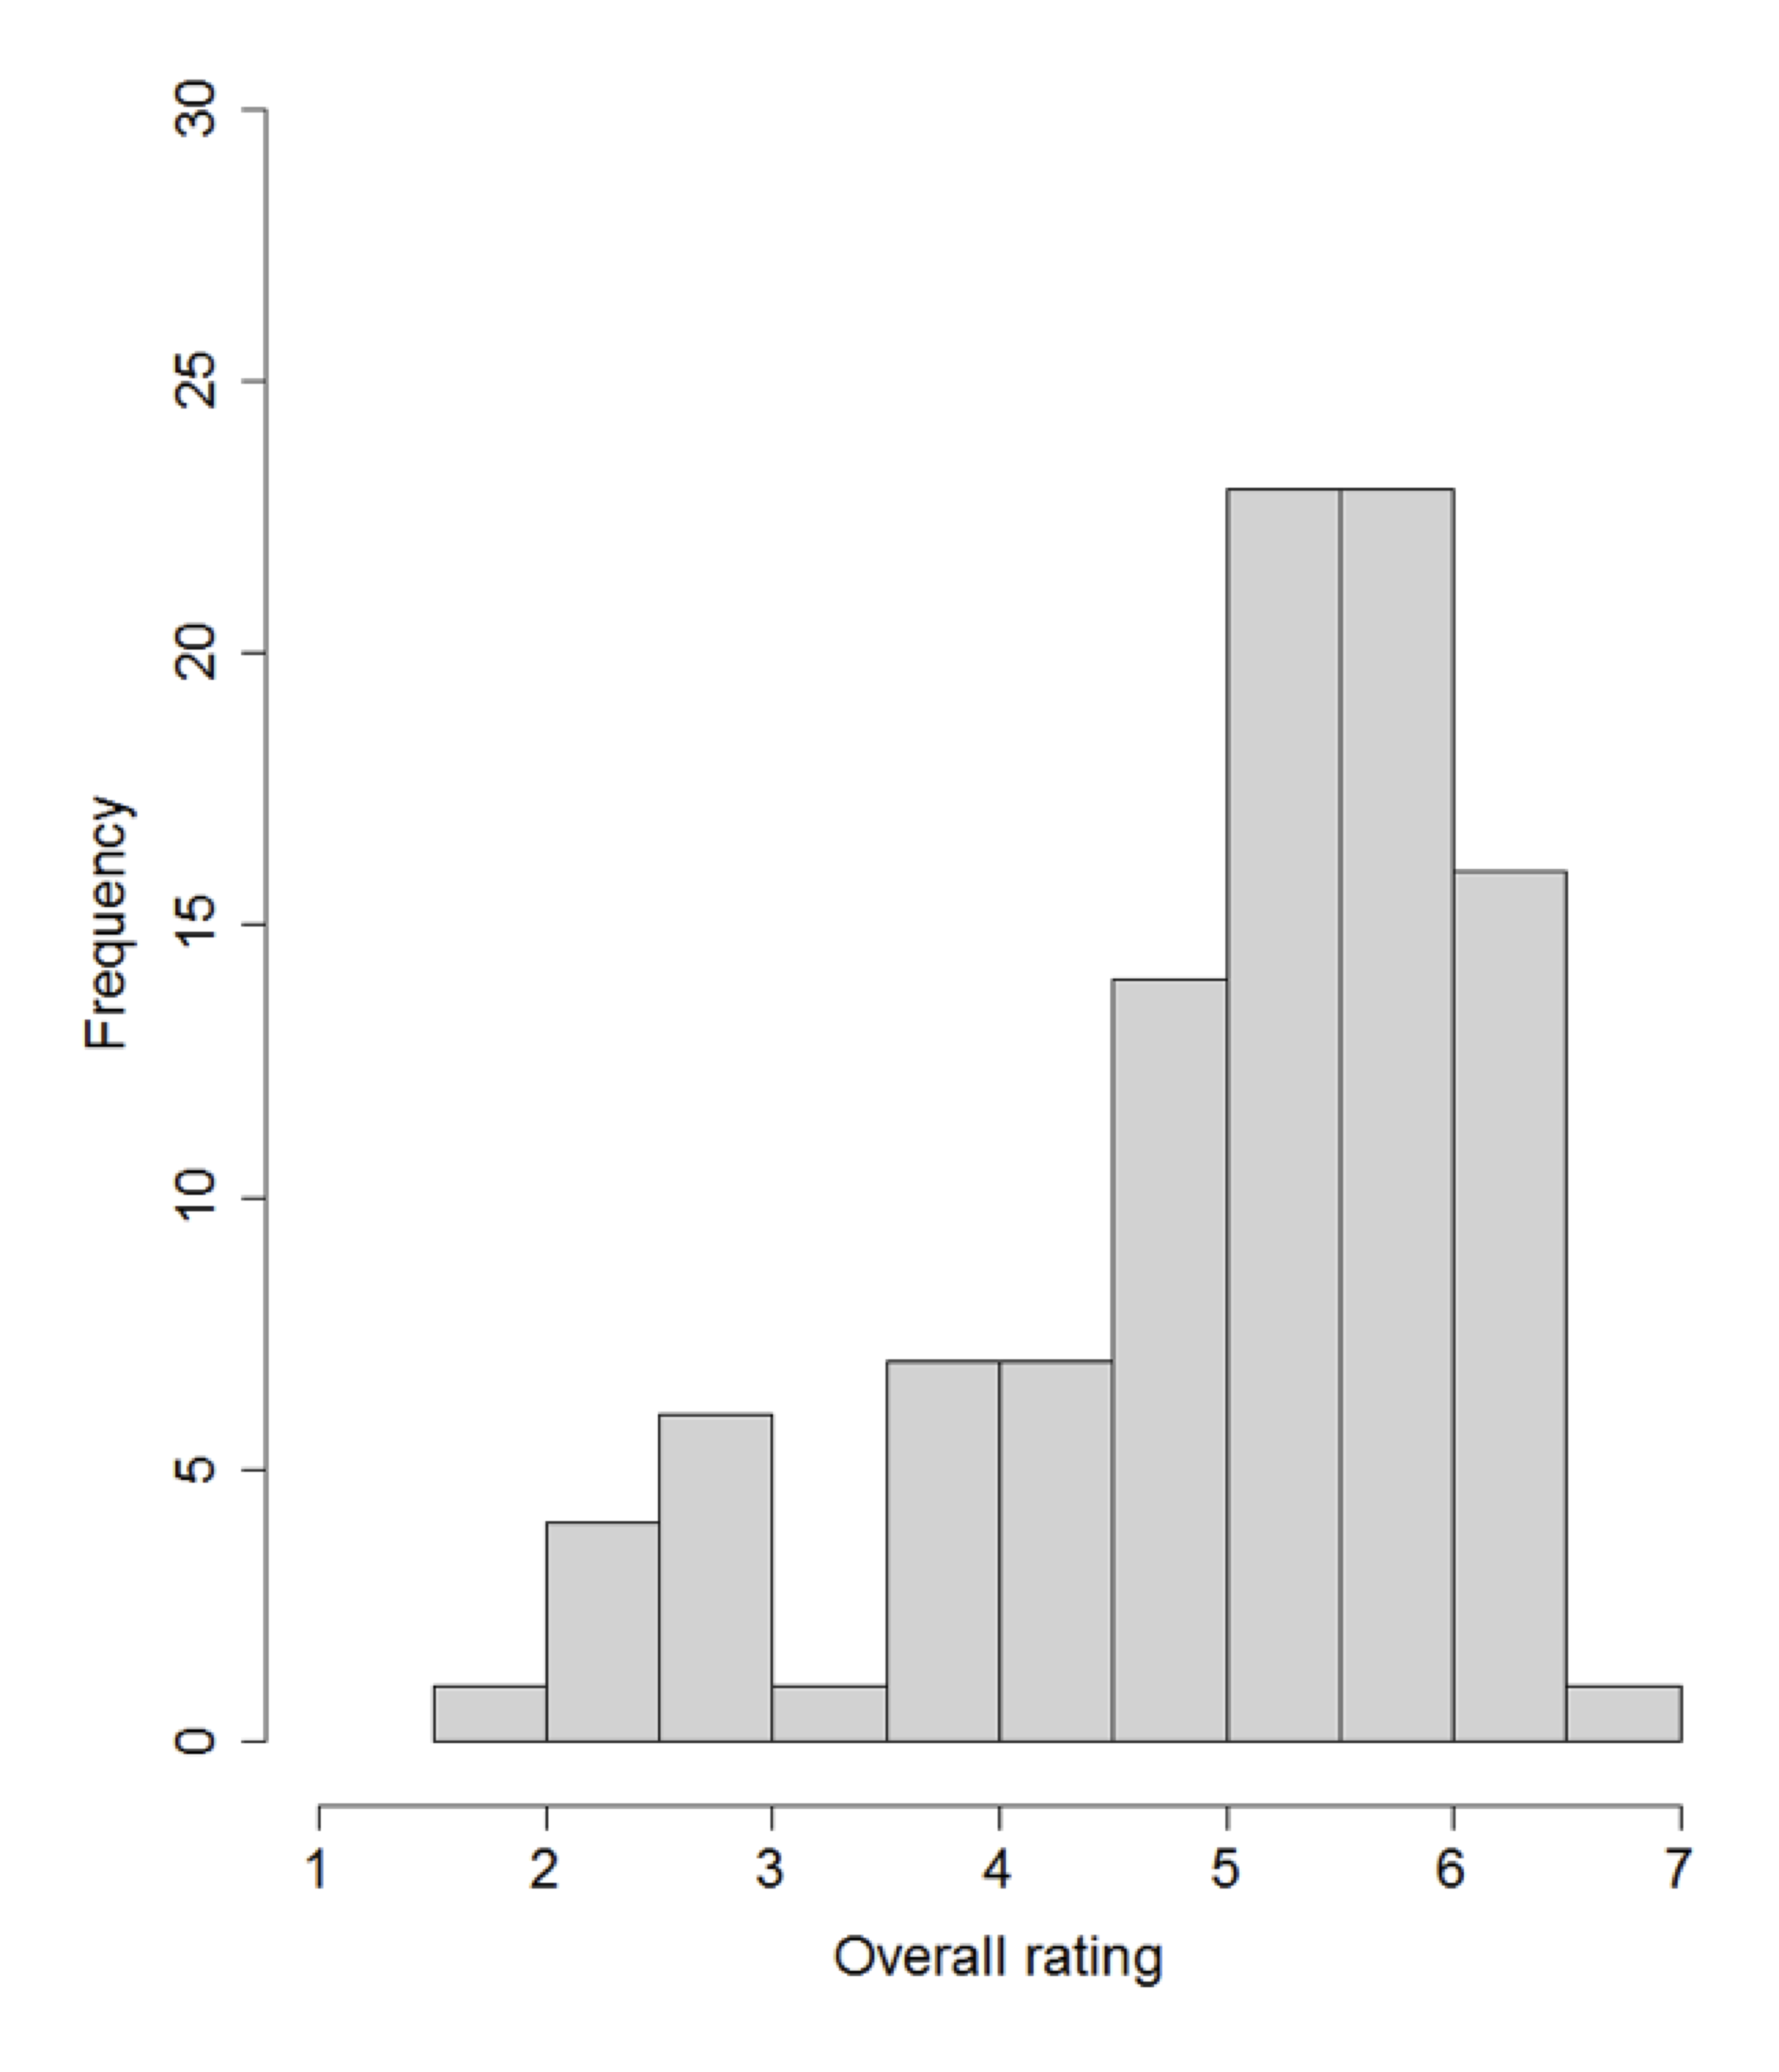
\includegraphics[width=0.45\linewidth]{pictures/overall}}
  \caption{Histogram of averaged ratings for the 103 different trajectories. Clockwise from top left: Efficient vs. Inefficient, Elegant vs. Inelegant, Smooth vs. Rough, Overall Rating}
\label{fig:survey_raw}
\end{figure}


An analysis of the ratings for each trajectory showed that four (averaged) ratings for each individual trajectory were always similar to each other, indicating that users had similar preferences for each trajectory regardless of the individual attributes used to describe the preference for the trajectory (efficient, elegant, smooth). 

Confidence intervals for the overall rating of each trajectory are shown in Fig.~\ref{confidence}. The small spread in the confidence intervals clearly indicates that different users had similar opinions about the same trajectory. Indeed, we found little evidence of any personal preference or clustering of users based on their preference for certain trajectories over others. 

\subsection{Feature Design for Trajectory Classification}

\todo 

Write about:
\begin{itemize}
\item clearance
\item smoothness
\item hausdorff distance
\item dynamic time warping
\item angular distance
\item path length
\item bfs path computation
\item figures for examples of high-low values of the above
\end{itemize}
\todo

\addtolength{\textheight}{-12cm}   % This command serves to balance the column lengths
                                  % on the last page of the document manually. It shortens
                                  % the textheight of the last page by a suitable amount.
                                  % This command does not take effect until the next page
                                  % so it should come on the page before the last. Make
                                  % sure that you do not shorten the textheight too much.

%%%%%%%%%%%%%%%%%%%%%%%%%%%%%%%%%%%%%%%%%%%%%%%%%%%%%%%%%%%%%%%%%%%%%%%%%%%%%%%%



%%%%%%%%%%%%%%%%%%%%%%%%%%%%%%%%%%%%%%%%%%%%%%%%%%%%%%%%%%%%%%%%%%%%%%%%%%%%%%%%



%%%%%%%%%%%%%%%%%%%%%%%%%%%%%%%%%%%%%%%%%%%%
\section*{ACKNOWLEDGMENT}

The preferred spelling of the word �acknowledgment� in America is without an �e� after the �g�. Avoid the stilted expression, �One of us (R. B. G.) thanks . . .�  Instead, try �R. B. G. thanks�. Put sponsor acknowledgments in the unnumbered footnote on the first page.



%%%%%%%%%%%%%%%%%%%%%%%%%%%%%%%%%%%%%%%%%%%%
\bibliography{IEEEabrv,max,arjun}
\bibliographystyle{IEEEtran}



\end{document}
